\chapter{恒星作为量子光源}
\label{chap:e17}

\begin{chapteropening}
上一章我们把各种天体辐射机制翻译成了量子语言：黑体、热光、受激辐射各自对应怎样的光子统计。现在把这套语言对准夜空里最普通、也最可靠的一类源——恒星。它们的光球（photosphere）近似一块发着热光的表面，角直径落在毫角秒（milliarcsecond, mas）量级，亮星每秒送来的光子多到足以做相关测量。更妙的是，强度干涉（intensity interferometry）只测两台望远镜光强涨落的相关，直接读出 \(|V|^2\)，完全不要求它们之间保持光学相位。这一章要回答一个问题：当我们把恒星不再当成一个点，而当成一块有结构的发光表面时，边缘昏暗、快速自转、星盘、双星、脉动，这些物理各自会在 \(|V(B)|^2\) 曲线上刻下怎样一道可分辨的指纹？我们会一路回收第 \ref{chap:e10} 章的 van Cittert--Zernike 定理与均匀圆盘，和第 \ref{chap:e11} 章的角直径、多基线成像，把它们落到 VERITAS 对 \(\beta\) UMa、\(\gamma\) Cas 等真实恒星的观测上 \citep{1956Natur.177...27B,1974MNRAS.167..121H,1974iiia.book.....H,2020NatAs...4.1164A,2024MNRAS.529.4387A}。
\end{chapteropening}

\section{为什么恒星是最稳的标定场}
\label{sec:e17-why-stars}

先说一个直觉：要检验一把尺子准不准，你会拿一个"你大致知道尺寸、而且不会乱动"的东西去量它。恒星恰好就是量子天文学这把新尺子的理想标定物。光球在局部热平衡（local thermodynamic equilibrium, LTE）下发出近似黑体的连续谱，谱形和总流量都能用成熟的恒星大气模型描述；亮星足够亮，光子统计误差可以靠积分时间压下去；而它们的角直径正好落在可见光百米基线能分辨的窗口。第 \ref{chap:e16} 章已经讲过，这种热光在单个相干模式里满足 \(g^{(2)}(0)=2\)——光子成群到来，涨落是相干态的两倍。

但真实望远镜看到的 \(g^{(2)}(0)-1\) 远小于 1。原因是模式稀释（mode dilution）：一次测量里混进了大量空间、偏振、频率和时间模式，每个模式各自贡献一份独立的热涨落，平均下来对比度被压低。第 \ref{chap:e08} 章给出的定量表述是 Siegert 关系里的那个稀释因子 \(\zeta\)，它约等于"单个相干模式占据的时空体积除以探测器实际接收的时空体积"。放到恒星上，这不是抽象命题：Vega 的 photon-counting 强度干涉实验在零基线测得 \(\langle g^{(2)}\rangle=1.0034\pm0.0008\)，只比 1 高出千分之三；在约 \(2~{\rm km}\) 基线上则测不到显著相关，这与 Vega 约 \(3.3~{\rm mas}\) 的角直径完全相容——星太大，公里基线早已把它分辨掉，可见度落到接近零 \citep{2021MNRAS.506.1585Z}。这就是第 \ref{chap:e08} 章模式稀释在一颗真实恒星身上的样子。

\paragraph{强度相关直接给出平方可见度}
\label{sec:e17-g2-vis}

强度干涉测的是两台望远镜光强涨落的零延迟相关。对热光，扣除背景、做完时间移位归一化之后，这个相关的超额部分正比于天空亮度分布的一个傅里叶模的模平方：
\begin{equation}
  g^{(2)}_{ij}(0)-1 \;=\; |\gamma_{ij}|^2 \;\simeq\; \bigl|V(u_{ij},v_{ij})\bigr|^2 .
  \label{eq:e17-g2-vis}
\end{equation}
\begin{formulaexplain}
\(g^{(2)}_{ij}(0)\)：望远镜 \(i,j\) 的零延迟强度相关。\(\gamma_{ij}\)：两台望远镜间的复相干度。\(V\)：归一化复可见度，\((u,v)\) 是投影基线除以波长。这条式子说：热光的强度相关超额，就是天空亮度傅里叶模的模平方。
\end{formulaexplain}
逐个交代符号。\(g^{(2)}_{ij}(0)\) 无量纲，是把两路光电流（或光子计数）在同一时刻相乘、再对各自平均归一化的结果，第 \ref{chap:e08} 章已推导过它对热光取 2、对相干态取 1。\(\gamma_{ij}\) 是复相干度，模在 0 到 1 之间；\((u,v)=\bm{B}_\perp/\lambda\) 是把投影基线 \(\bm{B}_\perp\)（单位 cm）除以波长 \(\lambda\)（单位 cm）得到的空间频率，量纲是"每弧度多少个波长"，也就是每弧度的条纹数。式 \eqref{eq:e17-g2-vis} 的左边来自真实数据处理——延迟直方图、时间移位背景扣除、归一化相关；右边则是纯几何的天空亮度傅里叶变换。关键在于：右边取了模平方，复相位彻底丢失。这意味着 \(|V|^2\) 对天空图像的整体平移和镜像翻转都不敏感（平移只改变傅里叶相位、镜像取共轭，模平方都看不出来）。但只要目标结构本身有确定的几何——一个圆盘的直径、一个椭圆的轴比、一对双星的间距——这些量仍然能从 \(|V|^2\) 精确读出。这正是本章后面每一节要做的事。

\paragraph{基线长度与角尺度是同一把标尺}
\label{sec:e17-baseline}

要分辨一个角尺度为 \(\theta\) 的结构，需要多长的基线？答案来自 van Cittert--Zernike 定理里最朴素的量纲关系：
\begin{equation}
  B \;\sim\; \frac{\lambda}{\theta}
  \;\simeq\; 103~{\rm m}
  \left(\frac{\lambda}{500~{\rm nm}}\right)
  \left(\frac{\theta}{1~{\rm mas}}\right)^{-1}.
  \label{eq:e17-baseline}
\end{equation}
\begin{formulaexplain}
\(B\)：所需基线长度。\(\lambda\)：观测波长。\(\theta\)：目标角尺度。可见光下，毫角秒的恒星对应百米基线，公里基线才够得着毫角秒以下的表面细节。
\end{formulaexplain}
把这个数量级算给自己看，才算真懂。取 \(\lambda=500~{\rm nm}=5\times10^{-7}~{\rm m}\)，\(\theta=1~{\rm mas}\)。1 mas 换成弧度要乘 \(4.848\times10^{-9}\)（因为 \(1~{\rm arcsec}=1/206265~{\rm rad}\)，再除以 1000），即 \(\theta=4.848\times10^{-9}~{\rm rad}\)。于是
\[
  B\sim\frac{\lambda}{\theta}=\frac{5\times10^{-7}~{\rm m}}{4.848\times10^{-9}}
  \approx 103~{\rm m}.
\]
这就是式 \eqref{eq:e17-baseline} 里那个系数 103 m 的来历。它告诉我们：一颗 \(1~{\rm mas}\) 的恒星，在可见光里要用百米基线才开始明显被分辨；而 \(0.1~{\rm mas}\) 的表面结构（比如自转扁率、星斑）需要公里量级的基线。历史上 Narrabri 强度干涉仪用 \(10\)--\(188~{\rm m}\) 的可变基线和两面 \(6.7~{\rm m}\) 反射面，测出了 32 颗亮星的角直径 \citep{1974MNRAS.167..121H,1974iiia.book.....H}。今天的 VERITAS、MAGIC 以及未来的 CTA 类阵列，用 \(>10~{\rm m}\) 口径的切伦科夫（Cherenkov）望远镜、更大的收光面积和数字相关器，重新打开了这个参数空间 \citep{2020NatAs...4.1164A,2024MNRAS.529.4387A}。

信噪比的标度已经在第 \ref{chap:e11} 章的式 \eqref{eq:e11-snr} 里给全了，这里只点名它对恒星选样的直接含义：光子率越高、电子带宽越大、积分越久，\(|V|^2\) 的误差越小（信噪比随积分时间只按平方根涨）；而背景光、探测器死时间、有限的时间分辨率和系统协方差决定了这种统计增益到哪里就"赚不动"了。所以第一批目标自然偏向亮、热、蓝、且角直径在百米基线上就能分辨的恒星 \citep{2013MNRAS.430.3187R,2020NatAs...4.1164A}。这句话不是口号，它是下一节"怎样布基线"的物理依据。

\section{怎样从平方可见度读出角直径和温度}
\label{sec:e17-diameter-teff}

从数据到半径，第一步是把恒星暂时当成一枚"均匀发光的硬币"——只有一个参数：角直径 \(\theta\)。这就是第 \ref{chap:e10} 章的均匀圆盘（uniform disk）模型，其可见度由式 \eqref{eq:e10-disk} 给出，
\[
  V_{\rm UD}(B)=\frac{2J_1(x)}{x},\qquad x=\frac{\pi\theta B}{\lambda},
\]
其中 \(J_1\) 是一阶贝塞尔函数，\(x\) 是无量纲的"分辨程度"。这里 \(B\) 是投影基线，\(\lambda\) 是有效波长，\(\theta\) 要用弧度（若以 mas 给出，乘 \(4.848\times10^{-9}\)）。强度干涉拟合的是 \(|V_{\rm UD}|^2\)，复相位已经被模平方抹掉。曲线上信息最密的地方是第一零点附近（\(x=3.8317\)，对应 \(B_0\approx1.22\lambda/\theta\)）——那里 \(|V|^2\) 对角直径最敏感；但零点附近 \(|V|^2\) 太小，背景和系统误差会盖过信号。所以实测要覆盖短、中、长三段基线：短基线固定总通量和相关归一化，中等基线给出直径的下降斜率，长基线检验模型是否还需要边缘昏暗、扁率或伴星。

\begin{figure}[tbp]
\centering
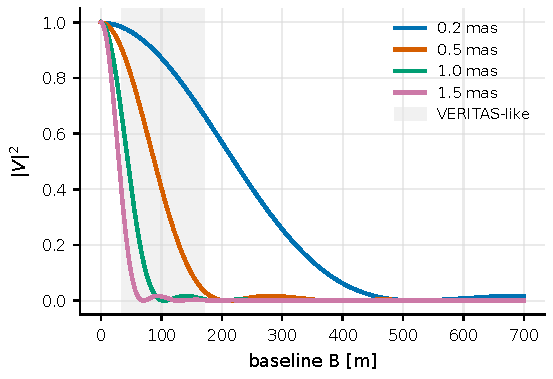
\includegraphics[width=0.82\linewidth]{figures/generated/chapter_10/ch10_stellar_diameter_visibility.pdf}
\caption{均匀圆盘恒星的 \(|V|^2\) 随基线变化。波长取 \(416~{\rm nm}\)，接近 VERITAS 强度干涉的观测波长。角直径越大，可见度下降得越快；灰色区域标出 \(35\)--\(170~{\rm m}\) 的 VERITAS 量级投影基线范围，适合测量约 \(0.5\)--\(1.5~{\rm mas}\) 的亮星。}
\label{fig:e17-diameter-visibility}
\end{figure}

\paragraph{角直径加总流量等于有效温度}
\label{sec:e17-teff}

量出角直径之后，只要再知道这颗星在地球处的总辐射流量，就能拿到它的有效温度（effective temperature）。推导只需要 Stefan--Boltzmann 定律加一步几何。恒星光度 \(L=4\pi R^2\sigma_{\rm SB}T_{\rm eff}^4\)，其中 \(R\) 是半径。传到距离 \(d\) 处，地球接收到的 bolometric flux 是 \(F_{\rm bol}=L/(4\pi d^2)=R^2\sigma_{\rm SB}T_{\rm eff}^4/d^2\)。而角直径与半径的关系是 \(\theta_{\rm LD}=2R/d\)，即 \(R/d=\theta_{\rm LD}/2\)，于是 \(R^2/d^2=\theta_{\rm LD}^2/4\)。代回去，距离 \(d\) 自动消掉：
\begin{equation}
  F_{\rm bol}=\frac{\theta_{\rm LD}^2}{4}\,\sigma_{\rm SB}T_{\rm eff}^4,
  \qquad
  T_{\rm eff}=\left(\frac{4F_{\rm bol}}{\sigma_{\rm SB}\theta_{\rm LD}^2}\right)^{1/4}.
  \label{eq:e17-teff}
\end{equation}
\begin{formulaexplain}
\(F_{\rm bol}\)：地球处测得的总辐射流量（\({\rm erg\,s^{-1}\,cm^{-2}}\)）。\(\theta_{\rm LD}\)：边缘昏暗角直径。\(\sigma_{\rm SB}\)：Stefan--Boltzmann 常数。角直径与总流量合起来，不需要知道距离就能定出有效温度。
\end{formulaexplain}
注意这个漂亮的地方：距离 \(d\) 在推导中被约掉了，所以 \(T_{\rm eff}\) 是一个"不依赖距离标尺"的量——你只需要测角直径和流量。\(\theta_{\rm LD}\) 下标 LD 提醒我们，这里该用边缘昏暗角直径（下一节解释为什么不能用均匀圆盘直径），单位是弧度或 mas；\(\sigma_{\rm SB}=5.67\times10^{-5}~{\rm erg\,s^{-1}\,cm^{-2}\,K^{-4}}\)（CGS）。

对同一颗星，我们更关心测量误差怎样传到 \(T_{\rm eff}\)。因为 \(T_{\rm eff}\propto F_{\rm bol}^{1/4}\theta_{\rm LD}^{-1/2}\)，取对数得 \(\ln T_{\rm eff}=\tfrac14\ln F_{\rm bol}-\tfrac12\ln\theta_{\rm LD}+{\rm const}\)。微分：\({\rm d}\ln T_{\rm eff}=\tfrac14\,{\rm d}\ln F_{\rm bol}-\tfrac12\,{\rm d}\ln\theta_{\rm LD}\)。若 \(F_{\rm bol}\) 与 \(\theta_{\rm LD}\) 的误差独立，方差按平方相加，系数取平方：
\begin{equation}
  \left(\frac{\sigma_T}{T_{\rm eff}}\right)^2
  \simeq
  \frac{1}{16}\left(\frac{\sigma_F}{F_{\rm bol}}\right)^2
  +\frac{1}{4}\left(\frac{\sigma_\theta}{\theta_{\rm LD}}\right)^2 .
  \label{eq:e17-teff-error}
\end{equation}
\begin{formulaexplain}
\(\sigma_T,\sigma_F,\sigma_\theta\)：温度、总流量、角直径的绝对误差。因为 \(T_{\rm eff}\propto F_{\rm bol}^{1/4}\theta_{\rm LD}^{-1/2}\)，同样的百分比误差下，角直径那一项（系数 \(1/4\)）比流量那一项（系数 \(1/16\)）权重大四倍。
\end{formulaexplain}
系数 \(1/16=(1/4)^2\) 和 \(1/4=(1/2)^2\) 正是指数的平方。结论是：角直径的相对误差进入 \(T_{\rm eff}\) 的权重是流量的四倍，因此往往是角直径主导了温度的精度。这正是强度干涉的价值所在——它把一个原本靠模型间接推断的角直径，变成了直接测量。VERITAS 对 \(\beta\) Ursae Majoris（\(\beta\) UMa）的强度干涉观测给出 \(\theta_{\rm LD}=1.07\pm0.04\,({\rm stat})\pm0.05\,({\rm sys})~{\rm mas}\)，代进式 \eqref{eq:e17-teff} 得到 \(T_{\rm eff}\simeq9700\pm200\pm200~{\rm K}\)，还能进一步约束 Ursa Major 移动星群的年龄 \citep{2024ApJ...966...28A}。而 VERITAS 首次现代强度干涉巡测测的 \(\beta\) Canis Majoris（\(\beta\) CMa）和 \(\epsilon\) Orionis（\(\epsilon\) Ori）两颗亮蓝星，正是这套方法在真实天空里的开场 \citep{2020NatAs...4.1164A}。

\begin{figure}[tbp]
\centering
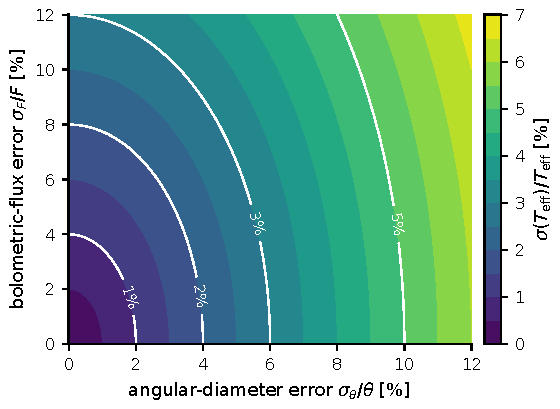
\includegraphics[width=0.78\linewidth]{figures/generated/chapter_10/ch10_teff_error_budget.pdf}
\caption{由 \(F_{\rm bol}\) 和 \(\theta_{\rm LD}\) 推导 \(T_{\rm eff}\) 的误差传播。横轴是角直径相对误差，纵轴是总流量相对误差，颜色给出有效温度相对误差。由于 \(T_{\rm eff}\propto F_{\rm bol}^{1/4}\theta_{\rm LD}^{-1/2}\)，角直径误差通常比同等百分比的流量误差更"值钱"。}
\label{fig:e17-teff-error}
\end{figure}

\paragraph{加上距离就得到半径和光度}
\label{sec:e17-radius}

如果这颗星的距离 \(d\) 由 Gaia 视差独立给出，那么角直径就能翻译成物理半径，Stefan--Boltzmann 定律再给出光度：
\begin{equation}
  R=\frac{1}{2}\theta_{\rm LD}\,d,\qquad
  L=4\pi R^2\sigma_{\rm SB}T_{\rm eff}^4 .
  \label{eq:e17-radius}
\end{equation}
\begin{formulaexplain}
\(R\)：恒星物理半径。\(d\)：距离。\(L\)：光度。角直径给出"天空上多大"，距离把它变成"实际多大"，再由 Stefan--Boltzmann 定律得到"发多亮"。
\end{formulaexplain}
第一式就是 \(\theta_{\rm LD}=2R/d\) 的改写；\(\theta_{\rm LD}\) 用弧度，\(d\) 与 \(R\) 同单位（比如都用 cm，或 \(d\) 用 pc、\(R\) 用 \(R_\odot\) 时记得换算）。把 Gaia 视差、强度干涉角直径和 \(F_{\rm bol}\) 三者联合，一颗恒星就落到赫罗（HR）图上一个带协方差的小区域里。这个小区域和恒星演化轨迹一比对，就约束了质量、年龄，以及混合长度、对流超射、自转等模型参数。红外流量法、Mark III 与 CHARA 等振幅干涉给出的角直径、以及强度干涉角直径，在这一层面是互相印证的独立标尺 \citep{1977MNRAS.180..177B,1991AJ....101.2207M,1994A&A...282..899B,2003AJ....126.2502M,2005ApJ...626..446R}。

\section{边缘昏暗为什么不是小修正}
\label{sec:e17-limb-darkening}

把恒星当均匀硬币，有一个必须还的债：真实恒星的圆面边缘更暗。原因很物理——当你看向圆盘中心时，视线垂直插进大气，看到的是较深、较热的层；当你看向边缘时，视线以很斜的角度掠过，只能看到较浅、较冷的高层。温度低，亮度就低，于是边缘发暗，这叫边缘昏暗（limb darkening）。最简单的线性模型是
\begin{equation}
  I(\mu)=I(1)\,[1-u_\lambda(1-\mu)],
  \qquad
  \mu=\sqrt{1-r^2}.
  \label{eq:e17-linear-ld}
\end{equation}
\begin{formulaexplain}
\(I(\mu)\)：不同视角处的表面亮度。\(\mu\)：表面法线与视线夹角的余弦。\(r\)：归一化投影半径（圆心 \(r=0\)，边缘 \(r=1\)）。\(u_\lambda\)：波长相关的边缘昏暗系数。它把"边缘变暗"压缩成一个参数。
\end{formulaexplain}
逐项看：\(r\) 是投影圆盘上的半径除以恒星半径，取值 0 到 1；圆心处视线垂直、\(\mu=1\)，边缘处视线掠射、\(\mu=0\)，几何关系正是 \(\mu=\sqrt{1-r^2}\)。\(I(1)\) 是圆心亮度。\(u_\lambda\) 是边缘昏暗系数，\(u_\lambda=0\) 退回均匀圆盘，\(u_\lambda\) 越大边缘越暗；它无量纲，且强烈依赖波长——热星在蓝光、冷巨星在分子吸收带、Mira 变星在不同脉动相位，\(u_\lambda\) 都不同。现代分析通常不用这条线性式，而是直接从大气模型生成合成的 \(I(\mu)\) 再算可见度；线性 \(u_\lambda\) 主要用来做数量级估算和直觉 \citep{1974MNRAS.167..475H,1992A&A...259..227D,1997A&A...327..199H,2015MNRAS.453.3821P}。

\paragraph{任意径向剖面的可见度是一次 Hankel 变换}
\label{sec:e17-hankel}

要知道边缘昏暗如何改可见度曲线，需要一个能吃"任意径向亮度剖面"的公式。对任何轴对称（圆对称）的亮度分布 \(I(r)\)，它的可见度就是径向的 Hankel 变换：
\begin{equation}
  V(x)=
  \frac{\displaystyle\int_0^1 I(r)\,J_0(xr)\,r\,{\rm d}r}
       {\displaystyle\int_0^1 I(r)\,r\,{\rm d}r},
  \label{eq:e17-hankel}
\end{equation}
\begin{formulaexplain}
\(V(x)\)：轴对称亮度分布的可见度。\(J_0\)：零阶贝塞尔函数。\(x\)：由基线、波长和角半径拼成的无量纲空间频率。分母是归一化（总通量），分子把亮度剖面投影到该频率上。
\end{formulaexplain}
这条式子从哪来？二维傅里叶变换对一个圆对称函数作用时，角向积分 \(\int_0^{2\pi}e^{-i x r\cos\phi}\,{\rm d}\phi=2\pi J_0(xr)\)——这是零阶贝塞尔函数的积分表示，是一个标准结果，直接把二维傅里叶变换降成一维径向积分。分母 \(\int_0^1 I(r)\,r\,{\rm d}r\) 是总通量，保证 \(V(0)=1\)。均匀圆盘是 \(I(r)={\rm const}\) 的特例：此时分子用到另一个标准结果 \(\int_0^1 J_0(xr)\,r\,{\rm d}r=J_1(x)/x\)，分母是 \(1/2\)，两者相除正好回到 \(V=2J_1(x)/x\)，即式 \eqref{eq:e10-disk}。把 \(u_\lambda>0\) 的线性剖面代进去，边缘变暗会让圆盘边界不再"尖锐"，效果是把可见度的第一零点往外推、并压低第一旁瓣的高度。

\begin{figure}[tbp]
\centering
\includegraphics[width=0.92\linewidth]{figures/generated/chapter_10/ch10_limb_darkening.pdf}
\caption{线性边缘昏暗对表面亮度和可见度的影响。左图显示 \(u_\lambda=0,0.4,0.8\) 三种情形下的径向亮度剖面；右图用式 \eqref{eq:e17-hankel} 数值积分得到相应的 \(|V|^2\)。边缘越暗，圆盘边界越模糊，可见度的零点和旁瓣位置随之移动。}
\label{fig:e17-limb-darkening}
\end{figure}

这正是为什么边缘昏暗不是"画图细节"，而是系统误差的来源：同一组 \(|V|^2\) 数据，若用均匀圆盘去拟合，得到的是 \(\theta_{\rm UD}\)；若用带边缘昏暗的大气模型去拟合，得到的是更接近真实光球边界的 \(\theta_{\rm LD}\)，两者可以差百分之几。它改变的不是曲线好不好看，而是"你到底量的是哪个半径"。Narrabri 的角直径目录当年就必须把均匀圆盘直径修正成 limb-darkened 直径，才能进一步谈温度和半径 \citep{1974MNRAS.167..121H,1974MNRAS.167..475H}。对强度干涉而言，标定误差还要叠加星表角直径、相关器增益、时间同步、背景光和 \(|V|^2\) 协方差的共同影响——每一项都要单独记账。

\section{自转、双星和表面结构怎样进入可见度}
\label{sec:e17-rotation-binary}

到这里恒星还是个圆。现实中它可能被自转压扁、可能有个伴星、可能表面斑驳。这些结构会把非圆、非对称的信息写进 \(|V|^2\)，我们逐个来看它们的指纹长什么样。

\paragraph{快速自转：扁率与 gravity darkening}
\label{sec:e17-rotation}

一颗转得很快的恒星，离心力把赤道甩得鼓起来，光球从球变成扁球（oblate spheroid）。更微妙的是 gravity darkening（重力昏暗）：赤道鼓起后表面重力减小，那里的表面温度也随之降低，于是赤道比两极更暗、更凉。几何上的第一效应是投影成椭圆。若把投影光球近似为一个椭圆，那么沿基线方向 \(\psi\) 看到的有效角直径是
\begin{equation}
  \theta_{\rm eff}^2(\psi)=
  \theta_{\rm maj}^2\cos^2\psi+
  \theta_{\rm min}^2\sin^2\psi ,
  \label{eq:e17-ellipse}
\end{equation}
\begin{formulaexplain}
\(\theta_{\rm eff}(\psi)\)：基线方向 \(\psi\) 上看到的有效角直径。\(\theta_{\rm maj},\theta_{\rm min}\)：投影椭圆的长、短轴角直径。自转扁率让 \(|V|^2\) 的下降速度随位置角改变。
\end{formulaexplain}
这条式子就是椭圆在方向 \(\psi\) 上的"视宽度"公式：当基线沿长轴（\(\psi=0\)）时 \(\theta_{\rm eff}=\theta_{\rm maj}\)，星显得最"宽"，可见度掉得最快；沿短轴（\(\psi=90^\circ\)）时 \(\theta_{\rm eff}=\theta_{\rm min}\)，可见度掉得最慢。于是同样长的基线，指向不同位置角，会读出不同的 \(|V|^2\)——这就是扁率留下的可分辨指纹。VERITAS 在 \(416~{\rm nm}\) 对 \(\gamma\) Cassiopeiae（\(\gamma\) Cas）的强度干涉观测正是这样测到扁率的：短轴角直径 \(0.43\pm0.02~{\rm mas}\)，长短轴半径比 \(1.28\pm0.04\)，位置角 \(116^\circ\pm5^\circ\)；再用快速自转大气模型，进一步给出接近 breakup（解体自转极限）的自转速度下限和约 \(10.9~R_\odot\) 的赤道半径 \citep{2025ApJ...995..191A}。

\begin{figure}[tbp]
\centering
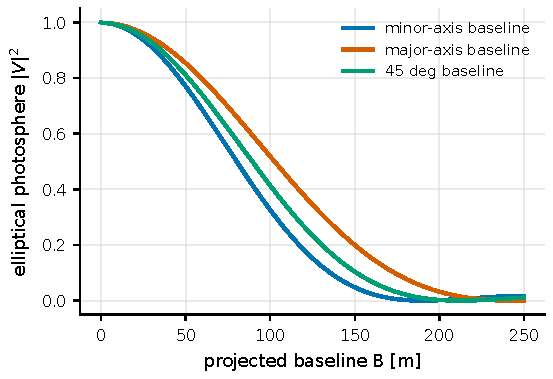
\includegraphics[width=0.82\linewidth]{figures/generated/chapter_10/ch10_rotation_oblateness.pdf}
\caption{快速自转椭圆光球在不同基线方向上的 \(|V|^2\)。参数取 \(\gamma\) Cas 量级的轴比 \(1.28\) 和 \(416~{\rm nm}\) 波长。沿不同位置角投影时有效角直径不同，因此同一基线长度给出的相关强度也不同；这一几何效应使强度干涉能直接测出光球扁率。}
\label{fig:e17-rotation}
\end{figure}

\paragraph{双星：可见度空间里的余弦振荡}
\label{sec:e17-binary}

一对靠得很近、各自都还没被分辨的双星，会在可见度曲线上叠一层余弦波纹。推导很直接：把两颗星当两个点源，主星流量取 1、次星取 \(f\)（流量比），角分离向量 \(\bm{d}\)。两个点源的可见度是各自复相位的加权和，\(V=(1+f\,e^{i\phi})/(1+f)\)，其中相位 \(\phi=2\pi\bm{u}\cdot\bm{d}\) 来自两点源的光程差。取模平方：\(|1+f e^{i\phi}|^2=(1+f\cos\phi)^2+(f\sin\phi)^2=1+f^2+2f\cos\phi\)。除以归一化 \((1+f)^2\)：
\begin{equation}
  |V_{\rm bin}|^2=
  \frac{1+f^2+2f\cos(2\pi\bm{u}\cdot\bm{d})}
       {(1+f)^2}.
  \label{eq:e17-binary}
\end{equation}
\begin{formulaexplain}
\(|V_{\rm bin}|^2\)：未分辨双星的平方可见度。\(f\)：次星与主星的流量比。\(\bm{u}=\bm{B}_\perp/\lambda\)：空间频率。\(\bm{d}\)：角分离向量（弧度）。余弦项让双星在基线空间里振荡。
\end{formulaexplain}
读这条式子：振荡周期由 \(\bm{u}\cdot\bm{d}\) 决定，分离 \(\bm{d}\) 越大、沿基线投影越长，随基线振荡得越快，于是从振荡周期能反推出沿基线方向的角分离；振荡的深浅由 \(f\) 决定，当 \(f\to1\)（两星等亮）时余弦项系数 \(2f/(1+f)^2\to1/2\) 最大，波纹最深，\(f\to0\)（次星极暗）时波纹消失。若两颗星各自还被部分分辨，只需把各自的圆盘可见度式 \eqref{eq:e10-disk} 乘进对应项即可。Narrabri 目录里有些目标后来被认出是双星或多星；现代多基线强度干涉阵列可以把双星轨道、角直径和亮度比联合拟合，再结合径向速度定出质量 \citep{1970MNRAS.148..103H,1974MNRAS.167..121H,2012MNRAS.419..172N}。

\begin{figure}[tbp]
\centering
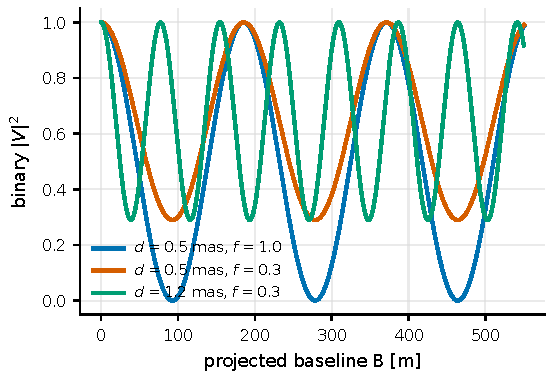
\includegraphics[width=0.82\linewidth]{figures/generated/chapter_10/ch10_binary_visibility.pdf}
\caption{未分辨双星的 \(|V|^2\) 振荡。角分离越大，随基线振荡越快；流量比越接近 1，振荡幅度越大。真实双星还需加入两颗星各自的有限角直径、轨道位置角和多波长流量比。}
\label{fig:e17-binary}
\end{figure}

\paragraph{表面结构：相位缺失带来的退化}
\label{sec:e17-surface}

表面结构比双星更棘手，因为 \(|V|^2\) 缺相位。星斑、对流大颗粒、非径向脉动、Be 星盘都会引入非轴对称的信号；如果只拿一个圆盘或双星模型去套，很可能得到一个"曲线拟合得很漂亮、但物理上是错的"结果——这正是相位缺失导致的模型退化。破解之道是增加约束维度：多基线、多个夜晚、多波长、以及谱线通道，都能各自压掉一部分退化。模拟研究表明，切伦科夫望远镜阵列凭借足够多的基线数和覆盖范围，有机会重建直径、扁率、双星结构乃至大尺度表面特征；但要重建真正复杂的图像，仍需要先验信息或与振幅干涉数据联合 \citep{2012MNRAS.419..172N,2013MNRAS.430.3187R}。

\section{时间变化和谱线通道怎样扩展恒星图像}
\label{sec:e17-time-line}

前面的星都是"静止"的。最后一节让恒星动起来、并让不同波长各说各话，看强度干涉还能多测出什么。

\paragraph{造父变星：把角半径变化接到距离标尺}
\label{sec:e17-cepheid}

造父变星（Cepheid）会周期性地一胀一缩，它的角直径随脉动相位变化。这给了一把独立于视差的量天尺——Baade--Wesselink 类方法。思路是：视向速度谱线告诉我们表面沿视线的运动速度，把它积分就得到半径的物理变化 \(\Delta R\)；而强度干涉直接测角半径的变化 \(\Delta\theta\)。两者之比就是距离。定量地，先约定符号：视向速度 \(v_r\) 以远离我们为正（红移为正），当表面朝我们膨胀时谱线蓝移、\(v_r-v_\gamma<0\)，而此时半径在增大，所以半径变化率与视向脉动速度差一个负号，
\[
  \frac{{\rm d}R}{{\rm d}t}=-p\,[v_r(t)-v_\gamma].
\]
两边对时间积分，得到半径的物理变化
\[
  \Delta R(t)=-\int p\,[v_r(t)-v_\gamma]\,{\rm d}t.
\]
再用角直径与半径的几何关系 \(\Delta\theta=2\Delta R/d\)，代入即得
\begin{equation}
  \Delta\theta(t)=-\frac{2}{d}
  \int p\,[v_r(t)-v_\gamma]\,{\rm d}t .
  \label{eq:e17-baade-wesselink}
\end{equation}
\begin{formulaexplain}
\(\Delta\theta(t)\)：角直径随时间的变化。\(d\)：距离。\(v_r-v_\gamma\)：扣掉整体系统速度后的视向脉动速度（远离为正）。\(p\)：把观测视向速度换算成真实脉动速度的投影因子。负号是速度正方向约定的结果；实际分析只关心 \(\Delta\theta(t)\) 的幅度与相位，符号由约定固定。
\end{formulaexplain}
逐项：\(v_r(t)\) 是谱线测得的视向速度，\(v_\gamma\) 是整颗星相对我们的系统速度（常数），二者之差才是脉动本身。式中的负号纯粹来自"视向速度以远离为正、而膨胀让表面朝我们靠近"这一符号约定；换一套约定负号就会翻面，真正做距离拟合时只用到 \(\Delta\theta(t)\) 曲线的形状（幅度和相位），因此负号不影响结果，但把它写对能保证正文推导和方框公式内部自洽。\(p\) 是投影因子（projection factor），因为谱线是对整个可见半球做视向速度加权平均，而我们要的是表面真实的径向膨胀速度，二者差一个约 \(1.3\) 量级的几何因子。角直径曲线 \(\Delta\theta(t)\) 与速度积分曲线相位匹配后，唯一的自由标度就是 \(d\)，于是距离被定出。系统误差来自 \(p\) 因子、边缘昏暗（脉动中 \(u_\lambda\) 会变）、伴星污染、周期变化和大气速度梯度。明亮造父在可见光强度干涉里特别诱人：它们既亮，半径变化又可预测 \citep{1997A&A...320..799F,2007A&A...476...73F}。

\paragraph{谱线通道：把连续谱和线区的结构分开}
\label{sec:e17-line}

Be 星和 Wolf--Rayet 星的连续谱来自光球，发射线却来自一层延展的星盘或星风，两者空间尺度不同。如果窄带滤光片同时框住连续谱和一条发射线，观测到的可见度是两者按通量加权的和：
\begin{equation}
  V_{\rm obs}=
  \frac{F_{\rm cont}V_{\rm cont}+F_{\rm line}V_{\rm line}}
       {F_{\rm cont}+F_{\rm line}} .
  \label{eq:e17-line-visibility}
\end{equation}
\begin{formulaexplain}
\(V_{\rm obs}\)：窄带内观测到的净可见度。\(F_{\rm cont},F_{\rm line}\)：连续谱与谱线的通量。\(V_{\rm cont},V_{\rm line}\)：各自的可见度。若连续谱已标定，就能反解出谱线形成区的可见度、进而其空间尺度。
\end{formulaexplain}
这条式子的物理根据是两个分量互不相干（mutually incoherent）：连续谱来自光球、发射线来自延展的星盘或星风，两者是不同区域、不同过程发出的光子，彼此没有固定相位关系。互不相干意味着它们的强度直接相加、交叉的干涉项在时间平均下为零，于是互相干函数（也就是可见度）按各自通量线性加权，得到式 \eqref{eq:e17-line-visibility}——无需假设场的相干叠加。用法很实在：先用相邻纯连续谱谱带定出 \(V_{\rm cont}\)（就是光球圆盘），再把它从式 \eqref{eq:e17-line-visibility} 里减掉，就反解出谱线区的 \(V_{\rm line}\)，进而约束星盘半径、倾角或星风几何。对快速旋转的 Be 星，H\(\alpha\) 谱线勾勒星盘，蓝光连续谱勾勒光球；\(\gamma\) Cas 就是范例——强度干涉直接测到光球扁率，而红外或 H\(\alpha\) 干涉补上星盘的几何 \citep{2025ApJ...995..191A}。

最后一类特殊情形是自然激光（astrophysical laser）和受激谱线，可能出现在 \(\eta\) Carinae 这类强辐射场与致密气体团块共存的系统里。要证明某条谱线来自受激辐射，光靠谱线强度不够；需要同时看线宽、空间位置、泵浦通道、偏振，以及谱线通道里的 \(g^{(2)}\)——受激辐射会把光子统计从热光的成群（\(g^{(2)}>1\)）推向相干态的泊松（\(g^{(2)}\to1\)）。第 \ref{chap:e16} 章讨论的自然激光量子诊断，在这里落地成了具体的目标选择清单 \citep{2004A&A...428..497J,2005NewA...10..361J,2008AIPC..984..216D}。

\section{本章要点}
\label{sec:e17-summary}

\begin{itemize}
  \item \textbf{恒星是最稳的标定场。}光球近似热光，亮星光子率足够，角直径在毫角秒量级；强度干涉直接读 \(|V|^2\)（式 \eqref{eq:e17-g2-vis}），不需要望远镜间保持光学相位。模式稀释使实测 \(g^{(2)}(0)-1\) 很小——Vega 零基线只测到 \(1.0034\pm0.0008\)。
  \item \textbf{基线与角尺度同一把尺。}\(B\sim\lambda/\theta\)：可见光下 \(1~{\rm mas}\) 对应约 103 m，\(0.1~{\rm mas}\) 的表面结构需要公里级基线（式 \eqref{eq:e17-baseline}）。
  \item \textbf{角直径加流量给温度。}\(F_{\rm bol}=(\theta_{\rm LD}^2/4)\sigma_{\rm SB}T_{\rm eff}^4\)，距离被约掉（式 \eqref{eq:e17-teff}）；角直径的相对误差在 \(T_{\rm eff}\) 里权重是流量的四倍（式 \eqref{eq:e17-teff-error}）。VERITAS 对 \(\beta\) UMa 得 \(\theta_{\rm LD}=1.07~{\rm mas}\)、\(T_{\rm eff}\simeq9700~{\rm K}\)。
  \item \textbf{边缘昏暗改的是"哪个半径"。}任意轴对称剖面的可见度是 Hankel 变换（式 \eqref{eq:e17-hankel}）；均匀圆盘直径 \(\theta_{\rm UD}\) 与边缘昏暗直径 \(\theta_{\rm LD}\) 可差百分之几，是系统误差而非画图细节。
  \item \textbf{自转、双星、表面结构各有指纹。}扁率让 \(|V|^2\) 随位置角变（式 \eqref{eq:e17-ellipse}，\(\gamma\) Cas 轴比 1.28）；双星叠一层余弦振荡（式 \eqref{eq:e17-binary}）；表面结构因相位缺失易退化，靠多基线、多波长、多夜晚破解。
  \item \textbf{时间与谱线扩展图像。}造父的角半径变化接上 Baade--Wesselink 定距离（式 \eqref{eq:e17-baade-wesselink}）；窄带里连续谱与谱线按通量加权（式 \eqref{eq:e17-line-visibility}），可分出光球与星盘。
\end{itemize}

\noindent\textbf{想一想。}
\begin{itemize}
  \item 一颗 \(0.5~{\rm mas}\) 的亮星，在 \(416~{\rm nm}\) 下第一零点大约在多长基线？（提示：\(B_0\approx1.22\lambda/\theta\)。）若你只有 \(35\)--\(170~{\rm m}\) 基线，你能不能到达零点？到不了对拟合角直径有什么影响？
  \item 若两颗等亮双星（\(f=1\)）的角分离沿某方向为 \(1~{\rm mas}\)，式 \eqref{eq:e17-binary} 的余弦项周期对应多长的基线间隔？把位置角转 \(90^\circ\) 后这个周期会怎样变？
  \item 为什么式 \eqref{eq:e17-teff} 里 \(T_{\rm eff}\) 不依赖距离，而式 \eqref{eq:e17-radius} 里的 \(R\) 和 \(L\) 却依赖？这对"先测温度还是先测半径"的观测策略意味着什么？
\end{itemize}
